\section{Robustness to Query Variations}
\subsection{Research Question 1: Reproduction}
A comprehensive set of experiments was conducted using the same datasets, models, and methodologies to evaluate the robustness of retrieval pipelines to query variations and investigate the extent to which the original study's findings can be successfully reproduced. The key results of the reproduction study are presented in this section.

The first objective was to assess the robustness of different ranking models to query variations, categorised into lexical traditional models (Trad), neural ranking models (NN), and transformer-based language models (TNN). The effectiveness of these models, when original queries were replaced with their corresponding query variations, was determined. The results are outlined in \tab{tab:ant-main-table} for ANTIQUE and in \tab{tab:trec-main-table} for TREC-DL-2019. These tables display the resulting nDCG@10 value for each method and model, grouped by their variation category.

\begin{table}[ht]
\centering
\caption{Effectiveness (nDCG@10) of each method and model for ANTIQUE when faced with different query variations. Bold indicates the highest values observed for each model. Subscripts, ↓/↑, signify statistically significant decreases/increases obtained through a two-sided paired Student's T-Test conducted at a 95\% confidence level when comparing the model's performance with the original queries.}
\label{tab:ant-main-table}
\resizebox{\columnwidth}{!}{%
\begin{tabular}{l|l|l|l|l|l|l|l|l}
\textbf{\textbf{Category}} & \textbf{\textbf{Variation Method}} & \textbf{\textbf{BM25}} & \textbf{\textbf{RM3}} & \textbf{KNRM} & \textbf{CKNRM} & \textbf{EPIC} & \textbf{BERT} & \textbf{T5} \\ \hline
- & Original Query & \textbf{0.2286} & \textbf{0.217} & 0.2181 & 0.2065 & 0.266 & \textbf{0.363} & \textbf{0.3333} \\ \hline
Misspelling & NeighbCharSwap & 0.1559↓ & 0.1469↓ & 0.159↓ & 0.1444↓ & 0.184↓ & 0.2608↓ & 0.2509↓ \\
Misspelling & QWERTYCharSub & 0.1613↓ & 0.1525↓ & 0.162↓ & 0.1553↓ & 0.192↓ & 0.2619↓ & 0.2652↓ \\
Misspelling & RandomCharSub & 0.1623↓ & 0.1593↓ & 0.1602↓ & 0.1476↓ & 0.1879↓ & 0.2563↓ & 0.2458↓ \\ \hline
Naturality & RemoveStopWords & 0.227 & 0.2161 & \textbf{0.2232} & \textbf{0.2153} & \textbf{0.2693} & 0.3391↓ & 0.32 \\
Naturality & T5DescToTitle & 0.1673↓ & 0.1646↓ & 0.1647↓ & 0.1672↓ & 0.2006↓ & 0.2402↓ & 0.2393↓ \\ \hline
Ordering & RandomOrderSwap & \textbf{0.2286} & 0.2169 & 0.2181 & 0.1978 & 0.2661 & 0.3566 & 0.3255 \\ \hline
Paraphrase & BackTranslation & 0.1618↓ & 0.1546↓ & 0.1609↓ & 0.1438↓ & 0.2032↓ & 0.274↓ & 0.2581↓ \\
Paraphrase & T5QQP & 0.2201 & 0.2063 & 0.2085 & 0.1957 & 0.2617 & 0.3389↓ & 0.3214 \\
Paraphrase & WordEmbedSynSwap & 0.1759↓ & 0.1715↓ & 0.1915↓ & 0.1689↓ & 0.2139↓ & 0.2809↓ & 0.2814↓ \\
Paraphrase & WordNetSynSwap & 0.1791↓ & 0.175↓ & 0.1933↓ & 0.1763↓ & 0.212↓ & 0.2829↓ & 0.2734↓ \\ \hline
\end{tabular}%
}
\end{table}
\begin{table}[ht]
\centering
\caption{Effectiveness (nDCG@10) of each method and model for TREC-DL-2019 when faced with different query variations. Bold indicates the highest values observed for each model. Subscripts, ↓/↑, signify statistically significant decreases/increases obtained through a two-sided paired Student's T-Test conducted at a 95\% confidence level when comparing the model's performance with the original queries.}
\label{tab:trec-main-table}
\resizebox{\columnwidth}{!}{%
\begin{tabular}{l|l|l|l|l|l|l|l|l}
\textbf{Category} & \textbf{Variation Method} & \textbf{BM25} & \textbf{RM3} & \textbf{KNRM} & \textbf{CKNRM} & \textbf{EPIC} & \textbf{BERT} & \textbf{T5}  \\ \hline
- & Original Query    & \textbf{0.4795} & \textbf{0.5156} &\textbf{ 0.4941} & \textbf{0.4931} & \textbf{0.624}  & \textbf{0.6358} & 0.6998  \\ \hline
Misspelling     & NeighbCharSwap   & 0.2747↓ & 0.2748↓ & 0.3078↓ & 0.308↓  & 0.3893↓ & 0.3812↓ & 0.4944↓ \\ 
Misspelling     & QWERTYCharSub    & 0.2435↓ & 0.2504↓ & 0.2563↓ & 0.2965↓ & 0.3496↓ & 0.3657↓ & 0.4461↓ \\ 
Misspelling     & RandomCharSub    & 0.2314↓ & 0.2347↓ & 0.2349↓ & 0.2263↓ & 0.295↓  & 0.3075↓ & 0.3963↓  \\ \hline
Naturality      & RemoveStopWords  & 0.4778 & 0.5113 & 0.4769 & 0.4756 & 0.6214 & 0.615  & 0.6862  \\ 
Naturality      & T5DescToTitle    & 0.4215 & 0.4344 & 0.3693↓ & 0.3928 & 0.5061↓ & 0.533↓  & 0.5717↓ \\ \hline
Ordering        & RandomOrderSwap  & \textbf{0.4795} & \textbf{0.5156} & \textbf{0.4941} & 0.4708 & 0.6227 & 0.6268 & 0.697  \\ \hline
Paraphrase      & BackTranslation  & 0.3964 & 0.4195 & 0.3954 & 0.3605↓ & 0.5301 & 0.4874↓ & 0.6058 \\ 
Paraphrase      & T5QQP            & 0.4722 & 0.5043 & 0.4525 & 0.4609 & 0.604  & 0.6222 & \textbf{0.7045} \\ 
Paraphrase      & WordNetSynSwap   & 0.3488↓ & 0.365↓  & 0.3615↓ & 0.3605↓ & 0.449↓  & 0.459↓  & 0.5457↓ \\ 
Paraphrase      & WordEmbedSynSwap & 0.353↓  & 0.3539↓ & 0.3767↓ & 0.368↓  & 0.4749↓ & 0.4816↓ & 0.5603↓  \\ \hline
\end{tabular}%
}
\end{table}

The findings reveal a substantial degree of alignment with the original study. The experiments consistently demonstrate a statistically significant decline in retrieval effectiveness when various query variations and model combinations are considered. For the TREC-DL-2019 dataset, this reduction is observed in 41 out of 70 instances, representing a slight deviation from the original study's results by 8 cases. Similarly, for the ANTIQUE dataset, a decrease in effectiveness is recorded in 51 instances, deviating by merely 3 cases from the original study's outcomes. Furthermore, the analysis of valid queries illustrates that, on average, the models experience a reduction in effectiveness of 22.02\% for TREC-DL-2019, a figure marginally distinct from the original study's 20.62\%. For ANTIQUE, the average decline amounts to 17.92\%, contrasting with the original study's 19.21\%. These consistent trends reaffirm the original study's pivotal assertion that retrieval pipelines exhibit limited robustness in the face of query variations. These outcomes substantiate previous evidence suggesting that query variations introduce considerable variability into diverse information retrieval systems.

Discrepancies emerge when comparing specific values between this study and the original research. On average, the discrepancies are less than 0.08; however, they are particularly evident in the results for the BERT model. One potential explanation for these differences is the value of training iterations. Although the exact training iteration value used in the original study remains undisclosed, when reproducing the study, a value of only 50 was used due to computational constraints. Notably, these minor deviations in results underline the intricate nature of replication work, where subtle variations in experimental settings, environmental conditions, or data pre-processing procedures can lead to distinctions in experimental outcomes.

The replication study effectively addresses Research Question 1 (RQ1). Through a meticulous replication of experiments and methodologies from the original study, critical insights have been offered, and the original findings fortified. The consistently corroborated results from the reproduction study underscore the limited robustness of retrieval pipelines in the face of query variations, consequently reinforcing the pivotal conclusion of the original study. This coherence in findings between the two independent studies signifies the robustness and broader applicability of the original study's observations. This outcome robustly attests to the validity of the research outcomes in the original study's context and their broader relevance, accentuating the significant role of query variations in evaluating retrieval systems.

\subsection{Research Question 2: Expansion}
To assess the generalisability of the original findings, the study replicated the experiments using the DL-TYPO dataset. Moreover, as the original study suggested that neural ranking models might not handle query variations well, even with modern datasets, DL-TYPO emerged as an apt candidate for testing the transference of this inquiry. The selection of DL-TYPO was motivated by its novel and unexplored nature, thereby substantiating its suitability for broadening the research.

\begin{table}[ht]
\centering
\caption{Effectiveness (nDCG@10) of each method and model for DL-TYPO when faced with different query variations. Bold indicates the highest value observed for each model. Subscripts, ↓/↑, signify statistically significant decreases/increases obtained through a two-sided paired Student's T-Test conducted at a 95\% confidence level when comparing the model's performance with the original queries.}
\label{tab:typo-main-table}
\resizebox{\columnwidth}{!}{%
\begin{tabular}{l|l|l|l|l|l|l|l|l}
\textbf{Category} & \textbf{Variation Method} & \textbf{BM25} & \textbf{RM3} & \textbf{KNRM} & \textbf{CKNRM} & \textbf{EPIC} & \textbf{BERT} & \textbf{T5} \\ \hline
- & Original Query    & 0.1911 & 0.1757 & \textbf{0.2117} & \textbf{0.1798} & 0.1862 & 0.1951↓ & 0.2882 \\ \hline
Misspelling     & NeighbCharSwap   & 0.1145 & 0.1086 & 0.1224↓ & 0.0961↓ & 0.0987↓ & 0.0865↓ & 0.1922  \\
Misspelling     & QWERTYCharSub    & 0.0772↓ & 0.0746↓ & 0.0813↓ & 0.0572↓ & 0.0707↓ & 0.0683↓ & 0.1139↓  \\
Misspelling     & RandomCharSub    & 0.068↓  & 0.0626↓ & 0.1083↓ & 0.079↓  & 0.0844↓ & 0.0733↓ & 0.148↓  \\ \hline
Naturality      & RemoveStopWords  & 0.1911 & 0.1757 & 0.2022 & 0.1666 & 0.1825 & 0.1762 & 0.2794  \\
Naturality      & T5DescToTitle    & 0.1347 & 0.1244 & 0.1351↓ & 0.1228 & 0.1434 & 0.1454 & 0.2055  \\ \hline
Ordering        & RandomOrderSwap  & 0.1911 & 0.1757 & \textbf{0.2117} & 0.1443 & 0.1875↓ & 0.1719 & 0.2707  \\ \hline
Paraphrase      & BackTranslation  & 0.1468 & 0.141  & 0.1578 & 0.121  & 0.1702 & 0.1625 & 0.2245  \\
Paraphrase      & T5QQP            & \textbf{0.2138} & \textbf{0.2052} & 0.1738 & 0.1546 & \textbf{0.1956} & \textbf{0.218} & \textbf{0.2897}  \\
Paraphrase      & WordEmbedSynSwap & 0.0809 & 0.075  & 0.106↓  & 0.0901↓ & 0.0976↓ & 0.0638↓ & 0.1326↓  \\
Paraphrase      & WordNetSynSwap   & 0.1097↓ & 0.0978↓ & 0.1255↓ & 0.1004↓ & 0.1033↓ & 0.1018↓ & 0.1726↓ \\ \hline
\end{tabular}%
}
\end{table}

\tab{tab:typo-main-table} displays the results for DL-TYPO when applying the same models and methodologies used in the original study. This table shows the resulting nDCG@10 value for each method and model, grouped by their variation category.

The primary objective was to ascertain if the conclusions regarding retrieval pipeline robustness held when confronted with this real query dataset. As anticipated, the results closely paralleled the original research with discernibly diminished effectiveness. A pronounced reduction in the retrieval models' performance manifested across most query variation scenarios, thus substantiating the initial investigation's findings. Notably, the extent of the overall effectiveness decline, averaging at 31.81\%, surpassed that observed for TREC-DL-2019 and ANTIQUE. This observation underscores the resilience of the conclusions derived from the original study when transposed to the novel and distinct DL-TYPO dataset. The research's core inferences and insights possess a certain degree of generalisability, albeit with the caveat of nuanced dataset-specific variations in the extent of the observed effects.

The variation in results between the DL-TYPO dataset and the previously studied datasets can be attributed to several underlying factors. Firstly, the DL-TYPO dataset inherently features more query variations (misspellings, specifically) than the synthetically generated counterparts. The diversity and unpredictability of these authentic query variations pose a more substantial challenge to the robustness of retrieval pipelines, leading to a potentially higher decline in effectiveness. Furthermore, the specific characteristics of the queries in the DL-TYPO dataset, such as the frequency and types of typos, differ significantly from those in the other datasets. These idiosyncrasies interact with the retrieval models and the query variations in a distinct manner, further contributing to variations in observed effectiveness.

As mentioned in the original study, dataset-specific properties, such as query lengths, language styles, and topical diversity, play a role in the differing outcomes. Additionally, the performance of retrieval models may also be influenced by the dataset's composition in terms of judged and unjudged documents. If the query variations in the DL-TYPO dataset significantly increase unjudged documents' ranking highly, this could impact the perceived effectiveness, even if some of these documents might be contextually relevant.

In comparing the performance of retrieval models on the DL-TYPO dataset to that on the ANTIQUE and TREC-DL-2019 datasets, it becomes evident that DL-TYPO exhibits a significant reduction in effectiveness when confronted with various query variations. This underperformance of DL-TYPO can be attributed to several factors, as discussed. 

\subsection{Robustness by Query Variation Category}
The approach employed in the original study was replicated to examine the impact of different query variation categories on model effectiveness. Four distinct categories, namely misspellings, paraphrasing, naturality, and ordering, were systematically assigned to various query variations. The distribution of nDCG@10 $\Delta$ values across all models and variation categories is illustrated in the accompanying \fig{fig:dist-plots}, and these results are substantiated by the mean nDCG@10 $\Delta$ values per category and dataset, as depicted in \fig{fig:cat-changes}.

\begin{figure}[ht]
    \centering
    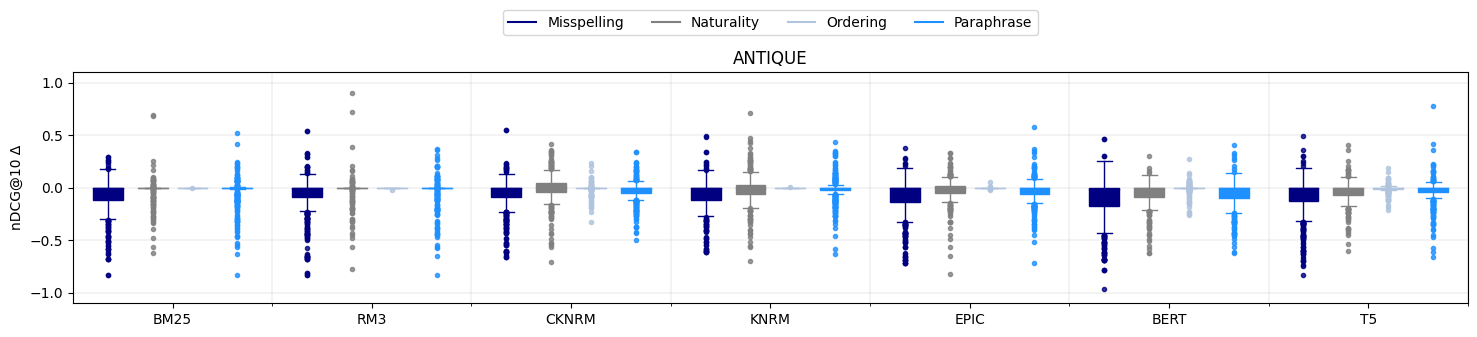
\includegraphics[width=1\linewidth]{5Results/main/plot_dist_antique.png}
    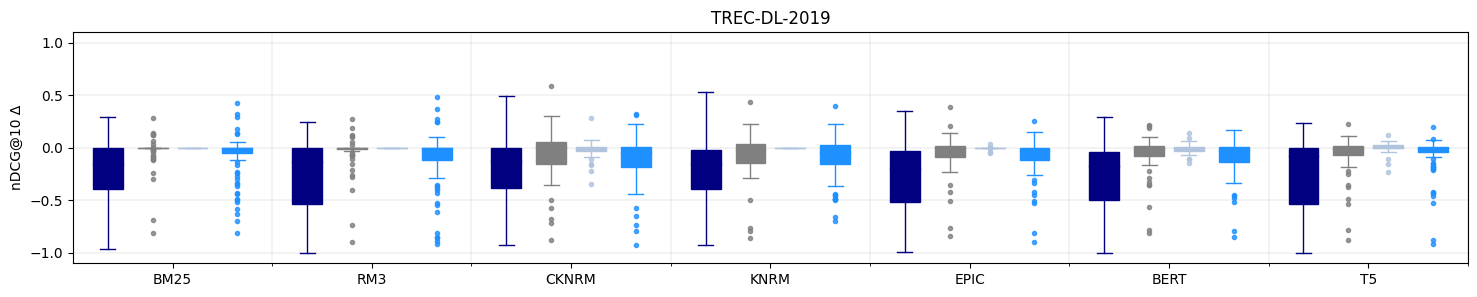
\includegraphics[width=1\linewidth]{5Results/main/plot_dist_trec.png}
    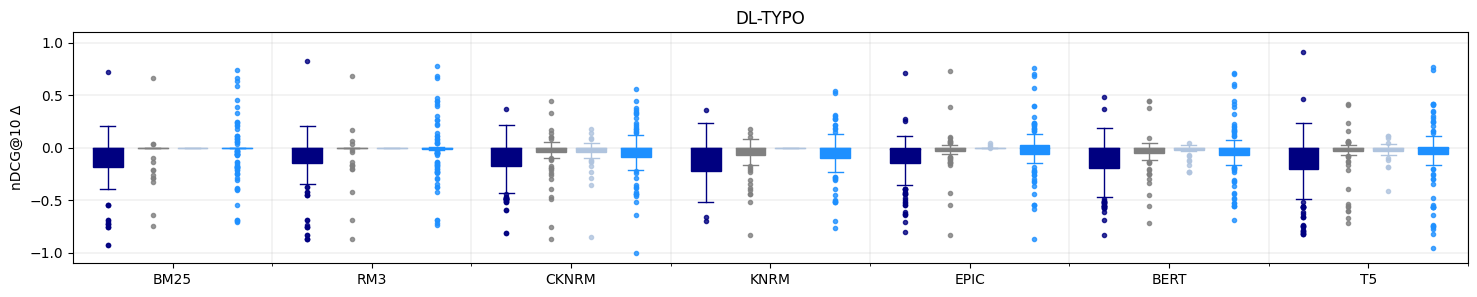
\includegraphics[width=1\linewidth]{5Results/main/plot_dist_dl-typo.png}
    \caption{Distribution of nDCG@10 $\Delta$ when replacing the original query by the methods of each category.}
    \label{fig:dist-plots}
\end{figure}

\begin{figure}[ht]
    \centering
    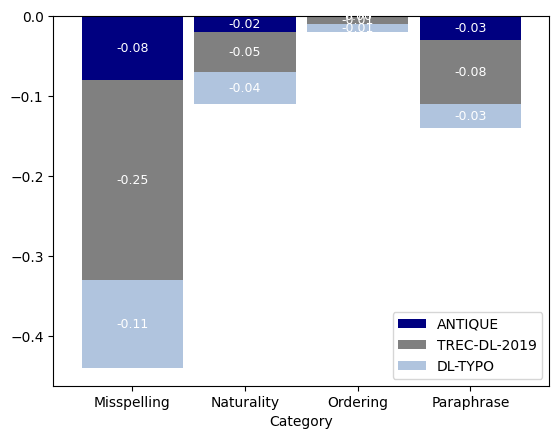
\includegraphics[width=0.8\linewidth]{5Results/main/plot_cat_changes.png}
    \caption{Average nDCG@10 $\Delta$ values per variation category for each dataset.}
    \label{fig:cat-changes}
\end{figure}

The findings highlight that, on average, the most pronounced negative impact was observed in misspelling variations. These variations recorded nDCG@10 $\Delta$ values of -0.08 for ANTIQUE, -0.25 for TREC-DL-2019, and -0.11 for DL-TYPO. These outcomes align with the observations made in the original study, further reinforcing the notion that misspelling variations consistently undermine retrieval effectiveness. In contrast, variations falling under the paraphrasing and naturality categories exhibited more modest nDCG@10 $\Delta$ values, with specific queries displaying a positive effect, mitigating the overall decline in retrieval performance. Notably, ordering variations had a negligible impact on traditional models, owing to their inherent nature as bag-of-words models, resulting in an average nDCG@10 $\Delta$ close to zero. This comprehensive evaluation elucidates the divergent impacts of distinct query variation categories on the efficacy of retrieval models. The consistent underperformance of DL-TYPO compared to ANTIQUE and TREC-DL-2019 further validates the notion that misspellings lead to diminished retrieval effectiveness. This is evident when comparing the original query values in \tab{tab:typo-main-table} with those in \tab{tab:ant-main-table} and \tab{tab:trec-main-table}.

\tab{tab:m-egs} provides an overview of how each of the methods affect the nDCG@10 $\Delta$ when applied to an example query from DL-TYPO. Notably, the T5DescToTitle method results in a significant reduction in nDCG@10 of 75\% . Other methods, such as NeighbCharSwap, RandomCharSub, and QWERTYCharSub, lead to approximately 49\% decreases in nDCG@10, underscoring their detrimental impact on query variations. This analysis emphasises the importance of carefully selecting variation methods, as their effects can vary significantly and have a substantial impact on the quality of retrieval results.

\begin{table}[ht]
\centering
\caption{Query variation and resulting change in effectiveness (nDCG@10 $\Delta$)  when we replace an example query from DL-TYPO with its variations for each variation method.}
\label{tab:m-egs}
\begin{tabularx}{\columnwidth}{l|X|l}
\textbf{Variation Method (M)} & \textbf{M("what does the declaration of independance represent")} & \textbf{nDCG@10 $\Delta$} \\ \hline
NeighbCharSwap  & what does the declaration of independance repreesnt  & -0.14 (-49.0\%) \\
RandomCharSub   & what does the declaration of independance represant  & -0.1 (-35.0\%)  \\
QWERTYCharSub   & what does the declaration of independance reprssent  & -0.14 (-49.0\%) \\ \hline
RemoveStopWords & declaration independance represent                   & -0.12 (-40.0\%) \\
T5DescToTitle   & declaration of independance                          & -0.22 (-75.0\%) \\ \hline
RandomOrderSwap & what does the declaration represent independance of  & -0.02 (-6.0\%)  \\ \hline
BackTranslation & what is the declaration of independence              & -0.14 (-49.0\%) \\
T5QQ            & what does the declaration of independence represent  & -0.05 (-17.0\%) \\
WordEmbedSynSwap    & what does the declaration of independance representing            & -0.04 (-15.0\%)           \\
WordNetSynSwap  & what does the announcement of independance represent & Invalid variation \\ \hline
\end{tabularx}%
\end{table}
